\documentclass{article}
\usepackage{graphicx} % Required for inserting images
\usepackage[a4paper, 
            left=3cm,    % Margen izquierdo 
            right=2.5cm, % Margen derecho (ligeramente menor)
            top=3cm,     % Margen superior
            bottom=3cm,  % Margen inferior
            headheight=15pt, % Espacio para encabezados
            footskip=1.5cm]  % Espacio para pies de página
           {geometry}
\usepackage[spanish,es-tabla]{babel}
\usepackage{float}



\title{Informe01_TICs_2025-01}
\author{JONATHAN IGNACIO FLORES TORRES}
\date{April 2025}

\begin{document}
\begin{titlepage}
\centering
\vspace{1cm}
{\Large UNIVERSIDAD DIEGO PORTALES \par}
\vspace{0.5cm}
{
\includegraphics[scale=0.5]{images/logo.png}\par}
\vspace{0.5cm}
{\scshape\Large FACULTAD DE INGENIERÍA Y CIENCIAS \par}

\vspace{3cm}
\centering
    \vspace*{1cm}
   \hrule height 0.5pt
\vspace{1mm}
\hrule height 1.5pt
\vspace{1cm}
{\scshape\Huge Informe 1 - Proyecto en TICs: AquiPhy \par}
\vspace{1cm}
\hrule height 1.5pt
\vspace{1mm}
\hrule height 0.5pt
\vspace{1.5cm}

\begin{tabular}{c}
    \textbf{Jonathan Flores} \\
        \textbf{Matias González} \\
    \textbf{Ilich Yévenes} \\
    \textbf{Profesor: Jorge Elliott} \\
    \textbf{Ayudante: Rafael Campos} \\
\end{tabular}

\vfill \today
\vspace*{1cm}
\end{titlepage}

\tableofcontents
\newpage
\section{Conformación de grupo y roles}

Para la distribución eficiente de tareas y actividades (definidas y señaladas posteriormente en el Plan de Trabajo), el equipo se ha dividido en dos grupos principales, considerando las habilidades y conocimientos de cada integrante:

\textbf{Grupo 1 - Hardware}:
Este grupo se encarga de la selección, adquisición y configuración de los sensores, así como del diseño y ensamblaje del circuito electrónico. Además, es responsable de la integración del hardware con el microcontrolador ESP32 y de la realización de pruebas de calibración para optimizar el consumo energético. Documentación y pruebas técnicas también forman parte de sus responsabilidades. Este grupo está conformado por Matias Gonzalez.

\textbf{Grupo 2 - Aplicación}:
Este grupo se centra en el desarrollo del firmware para la adquisición y procesamiento de datos. También es responsable de implementar la comunicación inalámbrica con la aplicación móvil, diseñar y desarrollar la interfaz de usuario para la visualización de datos, configurar el almacenamiento en la nube y gestionar las notificaciones. La documentación del código y las pruebas de integración también son parte fundamental de sus actividades. Este grupo está conformado por Ilich Yévenes y Jonathan Flores.
\section{Objetivos y Solución}

El agua es uno de los recursos naturales de mayor importancia que existe en nuestro planeta, pero debido a su mal uso y escasez comienzan a nacer diversas problemáticas derivadas de esto. Uno de los problemas que nos acompleja en mayor cantidad, es si el agua que usamos o consumimos realmente es apta para el fin a la que la vamos a destinar , y como podemos comprobar esto de manera simple y cotidiana. Es aquí donde nace la idea de AquiPhy.

Respecto al estudio y análisis de aguas se ha recopilado información de diferentes empresas y entidades para ocuparse como guía o inspiración, dentro de las cuales destacan las siguientes:

/////////

\textbf{-Aguas Andinas}: Aguas Andinas es la principal empresa en  
% desarrollo

\section{Motivación}

La calidad del agua está constantemente amenazada por factores como la contaminación industrial, el mal manejo de residuos y la falta de monitoreo accesible. A niveles locales, problemas como la alta concentración de cloro en el agua potable, acidificación o el desbalance de oxígeno en cultivos acuícolas demuestran la necesidad urgente de soluciones tecnológicas que permitan evaluar la calidad del agua de forma precisa, económica y en tiempo real.

Además, actualmente los equipos profesionales de análisis de agua son costosos y requieren cierto nivel de profesionalidad técnica, limitando su acceso al uso local/cotidiano, a pequeños agricultores o acuicultores. Por lo tanto, nuestro proyecto surge como una alternativa económica, innovadora y escalable, basada en el uso de Arduino y ESP32.

\section{Descripción del Problema}
% desarrollo

\section{Estado del Arte}
% desarrollo

\section{Idea de Artefacto y Diseño preliminar}

\subsection{Concepto General}
AquiPhy representa un avance significativo en la monitorización hidrológica inteligente, integrando tecnologías IoT con análisis de datos en tiempo real para ofrecer una solución completa de evaluación de calidad de agua. El sistema combina un dispositivo hardware basado en ESP32 con una suite de sensores especializados y una aplicación móvil con capacidades de inteligencia artificial, formando un ecosistema cerrado para la gestión hidrológica.

\subsubsection{Innovaciones clave:}

\begin{itemize}
    \item \textbf{Integración multisensor}: Capacidad para correlacionar hasta 7 parámetros fisicoquímicos simultáneamente.
    \item \textbf{Contextualización inteligente}: Motor de reglas adaptables que ajusta los umbrales de alerta según el uso específico (doméstico, acuícola, industrial).
\end{itemize}

\textbf{Flujo de operación:}
\begin{enumerate}
\item \textbf{Adquisición de datos}: Los sensores de alta precisión capturan parámetros del agua cada 5 segundos, con un jitter temporal menor a 50ms, garantizando consistencia en las mediciones.

\item \textbf{Procesamiento embebido}: El ESP32 ejecuta algoritmos de:
\begin{itemize}
    \item Compensación térmica (utilizando las lecturas del DS18B20 como referencia)
    \item Filtrado digital (media móvil ponderada de 5 muestras)
    \item Normalización dimensional (conversión a unidades estándar)
\end{itemize}

\item \textbf{Transmisión inalámbrica}: Los datos se envían mediante:
\begin{itemize}
    \item WiFi
    \item Bluetooth BLE (como respaldo en ausencia de red WiFi)
    \item Almacenamiento local en memoria flash (hasta 2 semanas de datos en caso de desconexión)
    \end{itemize}

\item \textbf{Interpretación contextual}: La aplicación móvil incorpora:
\begin{itemize}
    \item Base de conocimiento con perfiles preconfigurados
    \item Sistema experto para diagnóstico de problemas comunes
\end{itemize}

\item \textbf{Retroalimentación al usuario}: La capa de presentación ofrece:
\begin{itemize}
    \item Visualizaciones interactivas con zoom temporal
    \item Alertas codificadas por color (verde/amarillo/rojo)
    \item Recomendaciones accionables con procedimientos paso a paso
    \item Históricos comparativos (24h, 7d, 30d)
\end{itemize}

\item \textbf{Escalabilidad:} 
La arquitectura modular del sistema permite una fácil expansión y adaptación a nuevas necesidades. Esto incluye la incorporación de nuevos sensores a través de una configuración plug-and-play, así como la posibilidad de realizar actualizaciones tanto del firmware como de los perfiles de calidad, asegurando así una evolución continua del sistema sin necesidad de grandes modificaciones.

\end{enumerate}

\subsection{Aplicación Móvil}

La aplicación móvil constituye una herramienta esencial para el monitoreo y la gestión eficiente de la calidad del agua en tiempo real. Diseñada con un enfoque intuitivo y orientado al usuario, permite configurar perfiles personalizados, visualizar datos de manera clara y recibir alertas ante cualquier desviación de los parámetros establecidos. Esta solución tecnológica está pensada tanto para usuarios domésticos como para profesionales en áreas como acuicultura, gestión ambiental y tratamiento de agua potable.

\begin{itemize}
\item \textbf{Perfiles preconfigurados}: La aplicación incluye una variedad de perfiles diseñados para distintos usos, lo que facilita una configuración rápida y precisa sin necesidad de conocimientos técnicos avanzados.
  \begin{itemize}
  \item Acuarios tropicales: Parámetros óptimos como pH entre 6.5 y 7.5, y oxígeno disuelto mayor a 5\,mg/L, ideales para mantener especies sensibles en ambientes controlados.
  \item Agua potable: Control de cloro entre 0.2 y 4\,mg/L y turbidez inferior a 1\,NTU, garantizando condiciones seguras para el consumo humano.
  \item Acuicultura: Configuraciones específicas según el tipo de cultivo acuático.
    \begin{itemize}
    \item Peces de agua dulce: Requieren pH entre 6.5 y 8.5 y oxígeno mayor a 5\,mg/L, fundamentales para un crecimiento saludable.
    \item Camarones: Necesitan temperaturas entre 25--30$^\circ$C y oxígeno por encima de 4\,mg/L, condiciones críticas para su desarrollo.
    \item Salmónidos: Requieren altos niveles de oxígeno ($>6$\,mg/L) y bajas concentraciones de amoníaco ($<0.02$\,mg/L) para evitar estrés y mortalidad.
    \end{itemize}
  \end{itemize}
  
\item \textbf{Visualizaciones}: Permite una interpretación clara y dinámica de los datos recolectados mediante representaciones gráficas y esquemáticas.
  \begin{itemize}
  \item Gráficos temporales con tendencias: Ayudan a identificar patrones o anomalías en el comportamiento de los parámetros a lo largo del tiempo.
  \item Indicadores colorimétricos (verde/amarillo/rojo): Proveen una visualización rápida del estado de cada parámetro, facilitando la toma de decisiones inmediatas.
  \item Exportación CSV para análisis posterior: Ofrece la posibilidad de analizar los datos en herramientas externas como Excel, para generar reportes o realizar estudios más detallados.
  \end{itemize}
  
\item \textbf{Alertas inteligentes}: Un sistema automatizado que mejora la capacidad de respuesta ante situaciones críticas.
  \begin{itemize}
  \item Notificaciones push cuando parámetros salen de rango: El usuario recibe alertas en tiempo real directamente en su dispositivo móvil, lo que permite una intervención oportuna.
  \item Recomendaciones específicas para acuicultura: La app sugiere acciones correctivas basadas en el tipo de perfil configurado.
    \begin{itemize}
    \item ``Niveles de oxígeno bajos - activar aireadores'': Previene situaciones de hipoxia en el cultivo.
    \item ``pH elevado - considerar cambio parcial de agua'': Ayuda a restaurar condiciones óptimas del medio.
    \item ``Amoníaco detectado - verificar sistema de filtrado'': Minimiza el riesgo tóxico para las especies.
    \end{itemize}
  \end{itemize}
\end{itemize}



\section{Riesgos y Estrategias de Mitigación}

Es fundamental anticipar y gestionar los posibles riesgos que podrían afectar el desarrollo del proyecto, garantizando así el cumplimiento de los objetivos dentro del plazo establecido. A continuación, se detallan los principales riesgos identificados junto con las estrategias para mitigarlos y asegurar el éxito de este proyecto. 

\subsection{Riesgos}

\subsubsection{Dificultades técnicas inesperadas}
Durante el desarrollo del sistema de monitoreo de calidad de agua, podrían surgir complicaciones técnicas no previstas relacionadas con:

\begin{itemize}
    \item El diseño del circuito electrónico (interferencias, consumo eléctrico)
    \item Compatibilidad entre los diferentes sensores y el microcontrolador a utilizar
    \item Calibración precisa de los sensores químicos
    \item Estanqueidad del sistema para proteger los componentes electrónicos en ambientes húmedos
    \item Deriva de los sensores con el tiempo, requiriendo recalibraciones periódicas
\end{itemize}

Las dificultades técnicas representan el mayor riesgo en este tipo de proyectos. El ESP32, aunque potente, tiene limitaciones en el manejo de múltiples sensores simultáneos, especialmente cuando estos utilizan protocolos diferentes. La calibración de sensores químicos (como los de pH) requiere soluciones buffer de precisión y puede verse afectada por cambios de temperatura. Además, la exposición constante al agua exige un diseño cuidadoso de la carcasa para evitar cortocircuitos.

\subsubsection{Limitaciones del tiempo}
El proyecto cuenta con un plazo acotado para su desarrollo (3 meses), lo que podría generar:

\begin{itemize}
    \item Dificultades para implementar todas las funcionalidades planeadas
    \item Compromiso en la calidad final si surgen imprevistos
    \item Presión en las etapas de prueba y optimización
    \item Reducción del tiempo disponible para realizar pruebas de campo exhaustivas
\end{itemize}

El desarrollo de hardware embebido sufre frecuentes retrasos por problemas imprevistos. La integración de sensores comerciales con el ESP32 puede consumir tiempo valioso, especialmente cuando se requieren librerías personalizadas. Las pruebas de campo son cruciales pero demandan mucho tiempo, ya que se necesita esperar condiciones ambientales variantes para validar el comportamiento del sistema. Un cronograma realista debe incluir márgenes para resolver estos imprevistos.

\subsubsection{Desarrollo del firmware}
La programación del sistema podría presentar desafíos como:

\begin{itemize}
    \item Gestión simultánea de múltiples sensores con diferentes protocolos
    \item Procesamiento y filtrado de datos en tiempo real
    \item Consistencia en las transmisiones de datos mediante la nube o otro medio
    \item Implementación de algoritmos para compensación de temperatura en las lecturas
    \item Manejo de conexiones WiFi intermitentes y reconexión automática
\end{itemize}

El firmware es el cerebro del sistema y su desarrollo requiere atención especial. La lectura simultánea de sensores puede generar conflictos de timing, especialmente cuando algunos sensores tienen tiempos de respuesta largos. El procesamiento en tiempo real es esencial para proporcionar datos inmediatos, pero debe equilibrarse con el consumo energético. La transmisión a la nube debe implementar mecanismos de reintento y almacenamiento local para evitar la pérdida de datos durante fallos de conexión.

\subsection{Estrategias de Mitigación}

\subsubsection{Plan de contingencia técnica}
Las siguientes estrategias buscan anticipar y resolver problemas técnicos:

\begin{itemize}
    \item Pruebas semanales de integración para detectar problemas tempranos
    \item Identificación de componentes alternativos para elementos clave
    \item Considerar tiempo adicional para la recalibración de sensores
    \item Desarrollo de un prototipo en protoboard antes del diseño final
    \item Establecimiento de un protocolo de diagnóstico rápido de fallas
\end{itemize}

 Las pruebas de integración semanales seguirán un checklist que incluirá: comunicación sensor-microcontrolador, consumo energético y estabilidad de las lecturas. Se mantendrá una lista de componentes alternativos (como sensores equivalentes de diferentes fabricantes) para casos de disponibilidad o compatibilidad. Se asignará un 20\% adicional del tiempo total para calibraciones, considerando que sensores como los de pH requieren recalibración frecuente. El prototipo inicial permitirá verificar la viabilidad del diseño antes de comprometer recursos en la versión final.

\subsubsection{Gestión del cronograma}
Para garantizar el cumplimiento de los plazos:

\begin{itemize}
    \item Priorización de tareas críticas (adquisición de componentes, desarrollo del firmware, etc.)
    \item Reuniones semanales de seguimiento y ajuste de planificación
    \item Asignación de buffers de tiempo para tareas dependientes de proveedores externos
    \item Definición clara de hitos y entregables intermedios
\end{itemize}

 Se empleará un diagrama de Gantt con dependencias críticas, destacando en rojo las tareas que afectan la ruta crítica. Las reuniones semanales tendrán un formato estandarizado: revisión de avances (30\%), identificación de cuellos de botella (40\%) y reasignación de recursos (30\%). Los buffers de tiempo serán especialmente importantes para la adquisición de componentes importados, que pueden sufrir retrasos logísticos. Cada sprint culminará con un entregable funcional, aunque sea en versión beta.

\subsubsection{Enfoque en desarrollo de firmware}
Estrategias para garantizar un firmware robusto:

\begin{itemize}
    \item Implementación de simulaciones virtuales antes de pruebas físicas
    \item Pruebas por componente para cada módulo funcional
    \item Documentación detallada de cada implementación
    \item Capacitación para el uso de componentes/software específicos
    \item Desarrollo de casos de prueba para todas las funcionalidades
\end{itemize}

 Las simulaciones se realizarán en plataformas como \textit{Wokwi} para ESP32, permitiendo probar la lógica básica sin hardware físico. Cada módulo (comunicación con sensores, procesamiento de datos, transmisión WiFi) tendrá su propia suite de pruebas unitarias. La documentación incluirá diagramas de flujo, comentarios en el código y manuales de uso. Se dedicarán 4 horas semanales a capacitación en herramientas específicas como \textit{PlatformIO} (o otro tipo  de plataformas) o protocolos como \textit{Modbus} para sensores industriales. El control de versiones permitirá revertir cambios problemáticos fácilmente.

\newpage
\section{Plan de Trabajo}

El plan de trabajo incorpora el uso de software especializado en gestión de proyectos \textbf{ProjectLibre} para garantizar una planificación precisa y eficiente. Aprovechando las funcionalidades avanzadas de estas herramientas (diagramas de Gantt, gestión de dependencias entre tareas, seguimiento de hitos, etc.) se ha generado un cronograma dinámico que cubre todas las fases del proyecto. Este enfoque no solo optimiza la asignación de tiempos y responsabilidades, sino que también permite realizar ajustes ágiles ante imprevistos, manteniendo el flujo de trabajo alineado con los objetivos iniciales.

\begin{figure}[H]
    \centering
    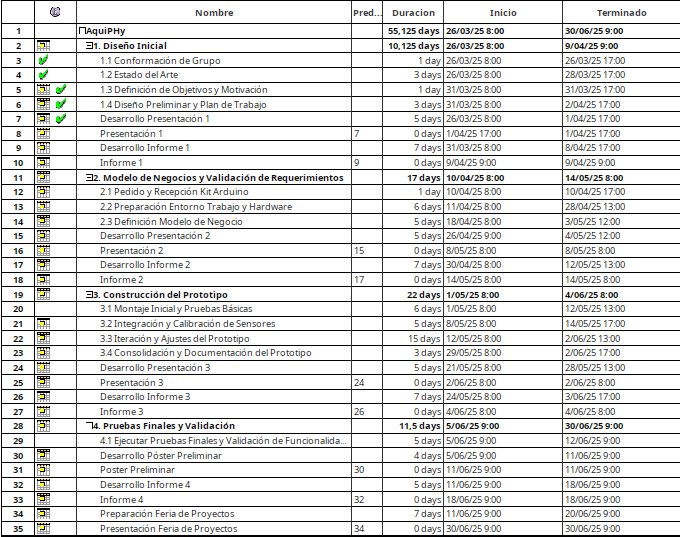
\includegraphics[width=.95\linewidth]{images/cartaGantt1of2.png}
    \caption{Lista de tareas y actividades en software \textit{ProjectLibre}.}
    \label{fig:cartaGantt1of2}
\end{figure}

De esta manera, se establecen de forma preliminar los responsables y los tiempos asignados para cada tarea. Posteriormente, el trabajo se consolida con el uso complementario de herramientas como Trello, que permite una organización incremental según la fase en desarrollo.

La Figura~\ref{fig:cartaGantt2of2} muestra una vista general del cronograma de trabajo para el desarrollo del proyecto durante el semestre, estructurado mediante un diagrama de Gantt y dividido en fases teóricas y prácticas, con entregables parciales (hitos) señalados con un cuadrado negro. Esta herramienta de gestión visual permite identificar claramente las fases críticas del proyecto, como el análisis de requisitos, desarrollo, pruebas y despliegue, junto con sus dependencias y hitos clave. La distribución temporal refleja una planificación equilibrada, asegurando así que el equipo cumpla con los plazos establecidos. 

\begin{figure}[H]
    \centering
    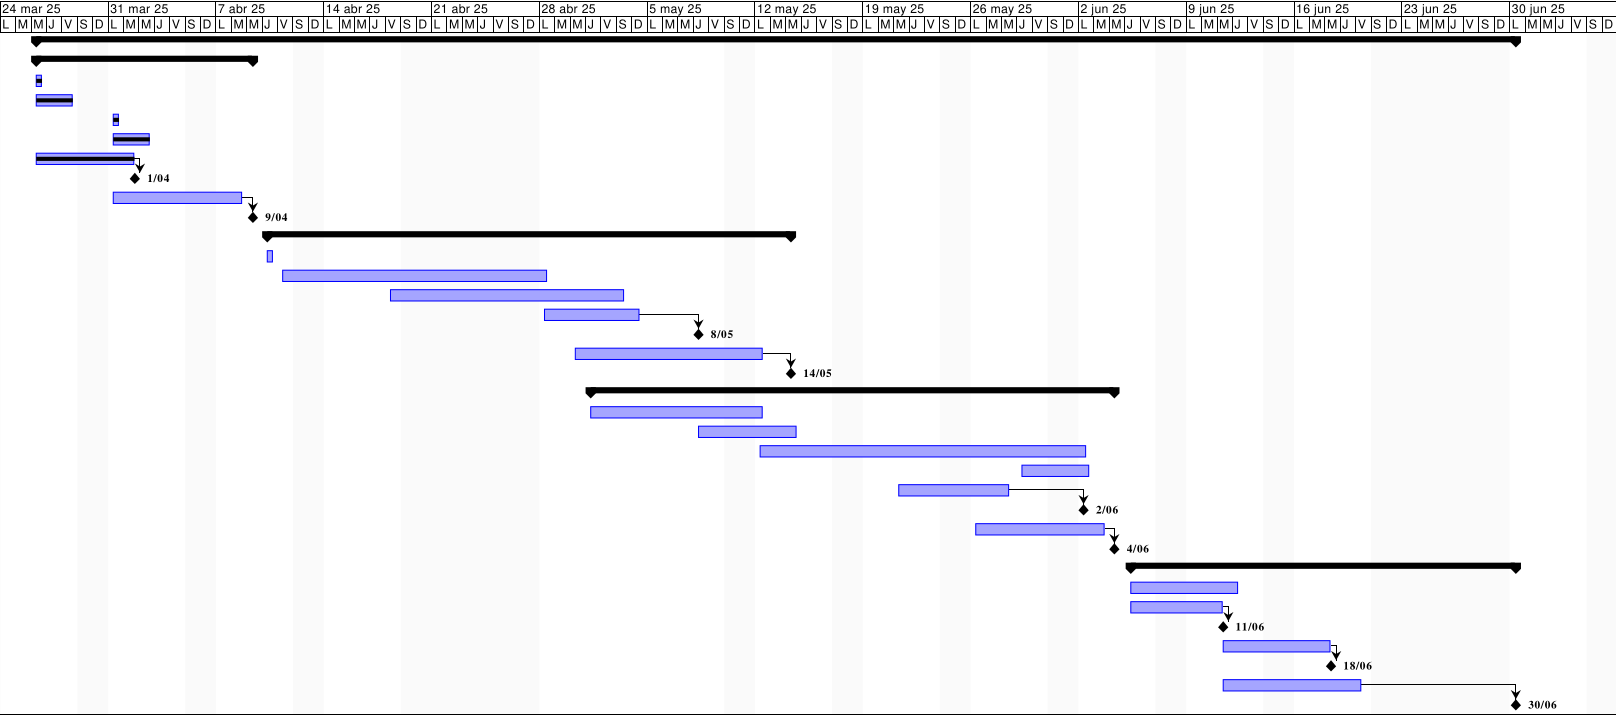
\includegraphics[width=.95\linewidth]{images/cartaGantt2of2.png}
    \caption{Vista general diagrama de Gantt en software \textit{ProjectLibre}.}
    \label{fig:cartaGantt2of2}
\end{figure}

\end{document}
